% Section 3.2 -- Recovering First-Layer Rows (role B)
\subsection{Recovering First-Layer Rows}
\label{sec:B-rows}

Each witness from Sect.~\ref{sec:A-critical} gives one row of $\Aone$, up to
scale and sign. Getting the row is easy in exact arithmetic. The real
difficulty is the finite-difference step: too small and rounding dominates,
too large and a probe crosses some hyperplane and the row is simply wrong.
Most of this subsection is about that step.

The idea is from~\cite[\S4.2]{DBLP:conf/crypto/CarliniJM20}. Where the
activation pattern is fixed, $f$ is affine with
$\nabla f(x)=\sum_{k}\Atwo_k\,\mathbb{1}[\pre{k}{x}>0]\,(\Aone_k)^{\top}$, so the
change of gradient across one critical hyperplane only contains that neuron.

\begin{proposition}[gradient jump]\label{prop:B-jump}
Let $x\in\wit{j}$, let $v$ be a unit vector with $\Aone_j v\neq0$, and let
$\delta>0$ be such that no other neuron changes sign on
$\{x+tv: |t|\le\delta\}$. Then
\begin{equation}\label{eq:B-jump}
  \nabla f(x+\delta v)-\nabla f(x-\delta v)
  =\operatorname{sign}(\Aone_j v)\,\Atwo_j\,(\Aone_j)^{\top}.
\end{equation}
\end{proposition}

\begin{proof}
For $k\neq j$ the indicator $\mathbb{1}[\pre{k}{\cdot}>0]$ is the same at both
points and cancels. $\pre{j}{x\pm\delta v}=\pm\delta\,\Aone_j v$, so $\eta_j$ is
active at exactly one of them, at $x+\delta v$ iff $\Aone_j v>0$. Only
$\Atwo_j(\Aone_j)^{\top}$ is left, with sign $\operatorname{sign}(\Aone_j v)$.\qed
\end{proof}

So the jump gives the direction of $\Aone_j$, nothing more. The length does not
matter (Proposition~\ref{prop:A-symmetry}); the sign does, and is fixed in
Sect.~\ref{sec:B-signs}. The bias of the unit row $\hat a$ is $\hat b=-\hat a\cdot x$,
since the witness lies on the hyperplane.

\paragraph{Algorithm.}
We estimate both gradients by forward differences along the $\dzero$ axes,
$\dzero+1$ queries per point, all in one batch (Algorithm~\ref{alg:B-row}).
Unlike~\cite[\S5.2]{DBLP:conf/crypto/CarliniJM20} we difference at points that
already sit on the two sides of the hyperplane. This keeps the relative signs
of the entries, so no column-sign step is needed.

\paragraph{The step must not cross the witness's own hyperplane.}
This was a real bug in our first version, and the exact witnesses used in
unit tests hide it. A probe $p_s+\varepsilon e_i$ is at distance
$\delta|\Aone_j v|/|\Aone_{j,i}|$ from $\wit{j}$ along $e_i$. When the search
line is nearly parallel to the hyperplane this is tiny, the probe crosses,
and the row comes out wrong. The bound
$\varepsilon<\delta/\sum_{i,j}|\Aone_{ij}|$ of~\cite[\S4.2]{DBLP:conf/crypto/CarliniJM20}
does not help: it needs the weights we are trying to find. Our fix costs one
extra query, $f(x)$. Along the line there is a single kink in
$[-\delta,\delta]$, so
$s_v=\bigl(f(p_{+})-2f(x)+f(p_{-})\bigr)/\delta$ is the exact slope jump along
$v$, and it must equal $J\cdot v$. If $|J\cdot v-s_v|>10^{-5}\|J\|$ we know a
probe crossed. We then take $|\hat a\cdot v|\approx|s_v|/\|J\|$ and redo the
differencing with
$\varepsilon\gets\min(10^{-2}\varepsilon,\;0.1\,\delta|s_v|/\|J\|_\infty)$.
On 3000 witnesses with uniformly random search directions, plain
differencing gave 28 wrong rows ($0.9\%$). With the check: none, at
$23.2$ queries per witness on average (\texttt{results/b\_rows\_lines.csv}).

\begin{algorithm}[t]
\caption{\texttt{row\_from\_witness}: one row of $\Aone$ (up to sign) from a witness.}
\label{alg:B-row}
\KwIn{oracle $\oracle$, witness $(x,v,r)$ with no other critical point within $\pm r$ along $v$}
\KwOut{unit row $\hat a$ and bias $\hat b$, or \texttt{None}}
$\delta\gets 0.1\,r$;\quad $\varepsilon\gets 0.01\,\delta$;\quad $p_{\pm}\gets x\pm\delta v$\;
$s_v\gets\bigl(\oracle(p_+)-2\oracle(x)+\oracle(p_-)\bigr)/\delta$\tcp*{reuses $\oracle(p_\pm)$; 1 query}
\Repeat{$|J\cdot v-s_v|\le10^{-5}\|J\|$ \textbf{or} 3 retries}{
  $g_{\pm}\gets\bigl(\oracle(p_\pm+\varepsilon e_i)-\oracle(p_\pm)\bigr)_{i=1}^{\dzero}/\varepsilon$
  \tcp*{$2(\dzero+1)$ queries}
  $J\gets g_{+}-g_{-}$;\quad $\varepsilon\gets\min(10^{-2}\varepsilon,\,0.1\,\delta|s_v|/\|J\|_\infty)$\;
}
\lIf{$J=0$}{\Return \texttt{None}\tcp*[f]{$\Atwo_j=0$: neuron invisible}}
$\hat a\gets J/\|J\|$;\quad \Return $(\hat a,\,-\hat a\cdot x)$\;
\end{algorithm}

\paragraph{No fixed step works.}
Rounding gives each partial derivative an error of about $u|f|/\varepsilon$
($u=2^{-53}$); relative to the jump $|\Atwo_j|\,\|\Aone_j\|$ that is a row error
of order $u|f|/(\varepsilon|\Atwo_j|\|\Aone_j\|)$. A large step instead crosses
another neuron's hyperplane and gives an $\Theta(1)$ error.
Fig.~\ref{fig:B-rows} shows both on 500 exact witnesses (\texttt{true\_witness},
50 networks). With a fixed $\varepsilon$ the median error falls like
$1/\varepsilon$, from $6.0\times10^{-6}$ at $10^{-10}$ to $7.2\times10^{-13}$ at
$10^{-3}$, but already from $\varepsilon\approx3\times10^{-6}$ the worst neuron
is off by more than $0.1$. So we tie the step to the witness radius,
$\varepsilon=10^{-3}r$. It never crossed a hyperplane; median error
$7.5\times10^{-12}$, worst $1.3\times10^{-8}$. The worst cases are neurons with
a small radius or a small $|\Atwo_j|$, as the estimate predicts, and
Sect.~\ref{sec:B-refine} cleans them up. On the test criterion all $1000$
neurons of $100$ networks have $|\cos(\hat a,\Aone_j)|\ge1-10^{-10}$, also with
search lines forced within $10^{-3}$ of parallel.

\begin{figure}[t]
\centering
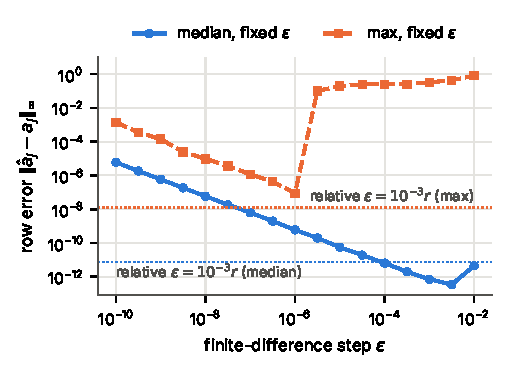
\includegraphics[width=0.75\linewidth]{figures/B/b_rows.pdf}
\caption{Row error after sign alignment versus the finite-difference step,
on 500 exact witnesses. Lines: fixed absolute $\varepsilon$; dotted: our
relative choice $\varepsilon=10^{-3}r$.}
\label{fig:B-rows}
\end{figure}

\paragraph{Merging.}
Several witnesses hit the same neuron, in no particular order. Two
candidates are one neuron if $|\cos(\hat a,\hat a')|>1-10^{-6}$. In a group we
flip everything to the first member's sign, average and renormalise the rows,
and take the median bias, so one bad witness cannot shift it. Fewer than
$\done$ groups: \texttt{merge\_neurons} returns \texttt{None} and the attack
searches another line. More than $\done$: the extra groups are spurious rows
(two close kinks taken as one) and we keep the $\done$ most frequent; a tie
at the cut also returns \texttt{None}, and \texttt{min\_count}$=2$ drops
singletons for signed weights. This is the duplicate filter
of~\cite[\S4.3.1]{DBLP:conf/crypto/CarliniJM20} without the deeper-layer part.
We do not need the graph clustering and median-of-ratios unification
of~\cite[\S5.4]{DBLP:conf/crypto/CarliniJM20}. That machinery handles partial
rows from hidden layers and the error blow-up from dividing by one small
entry. Here every witness gives a full row and we normalise by the Euclidean
norm, so $|\cos|$ is enough.

\paragraph{The coordinate method of~\cite[\S5.2]{DBLP:conf/crypto/CarliniJM20} is more precise but less safe.}
We implemented it as a bonus (\texttt{row\_from\_witness\_coord}). It steps
from $x$ itself along $\pm e_i$ and differentiates along the same axis. The
slope jump is then $|\Atwo_j|\,|\Aone_{j,i}|$, so the step can be large
($10^{-2}r$) but only magnitudes come out. Signs relative to the largest entry
$r$ come from the jump along $e_r+e_k$: $|a_r|+|a_k|$ for equal signs,
$\bigl||a_r|-|a_k|\bigr|$ otherwise. Total $1+2\dzero+2(\dzero-1)=39$ queries.
Table~\ref{tab:B-rowmethods} has the comparison. The coordinate method is
about ten times more precise at $1.7\times$ the queries, but it has nothing
that detects a crossed hyperplane, and it returned one wrong row out of 1000
random-direction witnesses. A wrong row breaks the whole extraction, while
the lost precision is recovered by Sect.~\ref{sec:B-refine}, so the attack
uses Algorithm~\ref{alg:B-row}.

\begin{table}[t]
\centering
\caption{Row recovery per witness on 100 $U[0,1]$ networks (errors after
normalisation and sign alignment; wrong: error $>10^{-5}$). Generated by
\texttt{experiments/b\_rows.py}.}
\label{tab:B-rowmethods}
\setlength{\tabcolsep}{4pt}
\begin{tabular}{llrrrr}
\toprule
method & witnesses & queries & median err. & max err. & wrong\\
\midrule
ours (Alg.~\ref{alg:B-row}) & exact & 23.0 & $6.1\times10^{-12}$ & $4.5\times10^{-8}$ & 0/1000\\
ours (Alg.~\ref{alg:B-row}) & search & 23.3 & $2.2\times10^{-12}$ & $6.6\times10^{-9}$ & 0/1000\\
coordinate~\cite[\S5.2]{DBLP:conf/crypto/CarliniJM20} & exact & 39.0 & $7.6\times10^{-13}$ & $4.4\times10^{-9}$ & 0/1000\\
coordinate~\cite[\S5.2]{DBLP:conf/crypto/CarliniJM20} & search & 39.0 & $2.4\times10^{-13}$ & $8.4\times10^{-2}$ & 1/1000\\
\bottomrule
\end{tabular}
\end{table}
